\section{Introduction}
\label{sec:intro}
Modern engineering design problems rely increasingly on the interdisciplinary interactions between subsystems. As a consequence, multidisciplinary design strategies have been developed, these allow to manipulate design variables from various disciplines simultaneously. Moreover, the incorporation of optimization tools within these methodologies leads to what is referred collectively as Multidisciplinary Design Optimization (MDO).    
The present work deals with the interaction of aerodynamics and structures, which is a key feature in aircraft design. Coupled aeroelastic analyses allow a better prediction of the aerodynamic forces and structural displacements that the aircraft experiences in real flight, hence, an MDO platform is implemented in order to study these interactions. \par 
Each discipline inside the MDO problem requires a solver that computes its effects on the global problem, with the aerodynamic effects being the main source of computational cost. High fidelity CFD analyses offer accurate results, but at the expense of high computational time. On the other hand, potential flow theory, and its computational implementation, the panel codes, offer reasonable approximations with low computational demands. The main goal of this project is to efficiently use low-fidelity analyses, combined to high-fidelity ones, to conduct aeroelastic optimizations, with an application to a Blended Wing Body (BWB) configuration.  
\section{State of the art}
\label{sec:state}
The starting point for the bibliography research is a Survey of Multifidelity Methods by Peherstorfer \cite{peherstorfer2018survey}, where a variety of alternatives are listed and classified. Surrogate modelling is a global optimization strategy. It uses co-kriging as a regression technique in order to link High-Fidelity sources with one or many Low-Fidelity functions. This correlated model can be used to find optimal solutions more quickly \cite{Forrester2007}. On the other hand, simpler approaches such as a linear regression are found to offer a good balance between accuracy, cost and simplicity \cite{Zhang2019}. Other advantages include: ease to combine many low-fidelity sources and robustness for High-Fidelity samples with the presence of noise \cite{Zhang2019}. \par
Newton methods and their variations have been explored as well. Jovanov and Breuker propose to solve the High-Fidelity problem by adding an aerodynamic correction load to the solution of the Low-Fidelity equation. The defect-correction method accelerates the convergence compared to the Quasi-Newton method \cite{Jovanov2015}. This last case does not consider the methods as black-boxes, but rather exploits the fact that the algorithms of both fidelity levels are known and can be modified at any stage to accommodate the necessary corrections between them. Scholz presents an Aggressive Space Mapping methodology, it solves for the low fidelity fluid–structure interaction solution and then feeds that information to a Quasi-Newton algorithm. The final results are obtained from a mapping function between both fidelity levels \cite{Scholcz2014}. \par
When it comes to the application of mutifidelity models to aerospace design, there are several publications on the subject. A Bayesian-enhanced Low-Fidelity correction proved the ability to maintain high-fidelity accuracy while reducing computational cost associated with the optimization of an airfoil shape \cite{fischer2018bayesian}. An aeroelastic optimization of a BWB was carried out by Bryson \cite{Bryson2019} using a modified Trust Region Model Management (TRMM) approach. Its main difference is that it adds hybrid additive-multiplicative corrections (or bridge functions) to the low-fidelity analysis \cite{Bryson2019a}. Another approach to the aeroelastic optimization of a BWB is presented by Marques \cite{Marques2019}. The flutter boundary problem is solved with a contour location approach (i.e. the zero contour of the aeroelastic damping coefficient). It also incorporates an active learning strategy, where the model evaluations are selected iteratively based on how much they are estimated to improve the predictions. \par

\section{Development}
\label{sec:development}
The starting point for the present method is the selection of the optimization platform and the structural and flow solvers. Given that the structural computation cost of the coupled aeroelastic problem is negligible compared to the High-Fidelity RANS algorithms for fluids, no multifidelity application is deemed relevant. In consequence, the well-known NASTRAN FEM implementation is chosen. On the other hand, the aerodynamic forces generated by the fluid on the structure will be computed using two fidelity levels: A Low-Fidelity panel code based on potential flow theory, PANAIR \cite{carmichael1981pan}; and a High-Fidelity CFD code, ADFlow, developed at the MDOlab \cite{lyu2013automatic}. \par
A multidisciplinary optimization platform is also needed in order to easily couple both parts of the problem and find the optimum design parameters. This project uses the OpenMDAO library developed at NASA's Glenn Research Center and coded in Python \cite{openmdao_2019}. Previous work in aeroelastic optimization using the aforementioned components has led to the development of a dedicated Python package: aerostructures \cite{mascolomer:tel-02023612}. This tool allows the user to easily create instances of common aerospace design problems within the OpenMDAO platform.\par
The aerostructures package includes a Low-Fidelity sample problem for a wing structure in typical cruise conditions \cite{vassberg2008development}. In addition to the two main disciplines (aerodynamics, structural), two other modules are required:
Load transfer, which assigns aerodynamic forces to the structural nodes while preserving the total load and moment; and displacement transfer, which interpolates the displacement field from the structural nodes to the aerodynamic points. Both modules use radial basis functions to allow the exchange of results between disciplines that do not share the same mesh topology. Based on the Low-Fidelity implementation, the same problem was programmed in High-Fidelity with the aim of creating a block of code that can be called by the multifidelity code once it is ready. 

\begin{figure}[H]
    \centering
    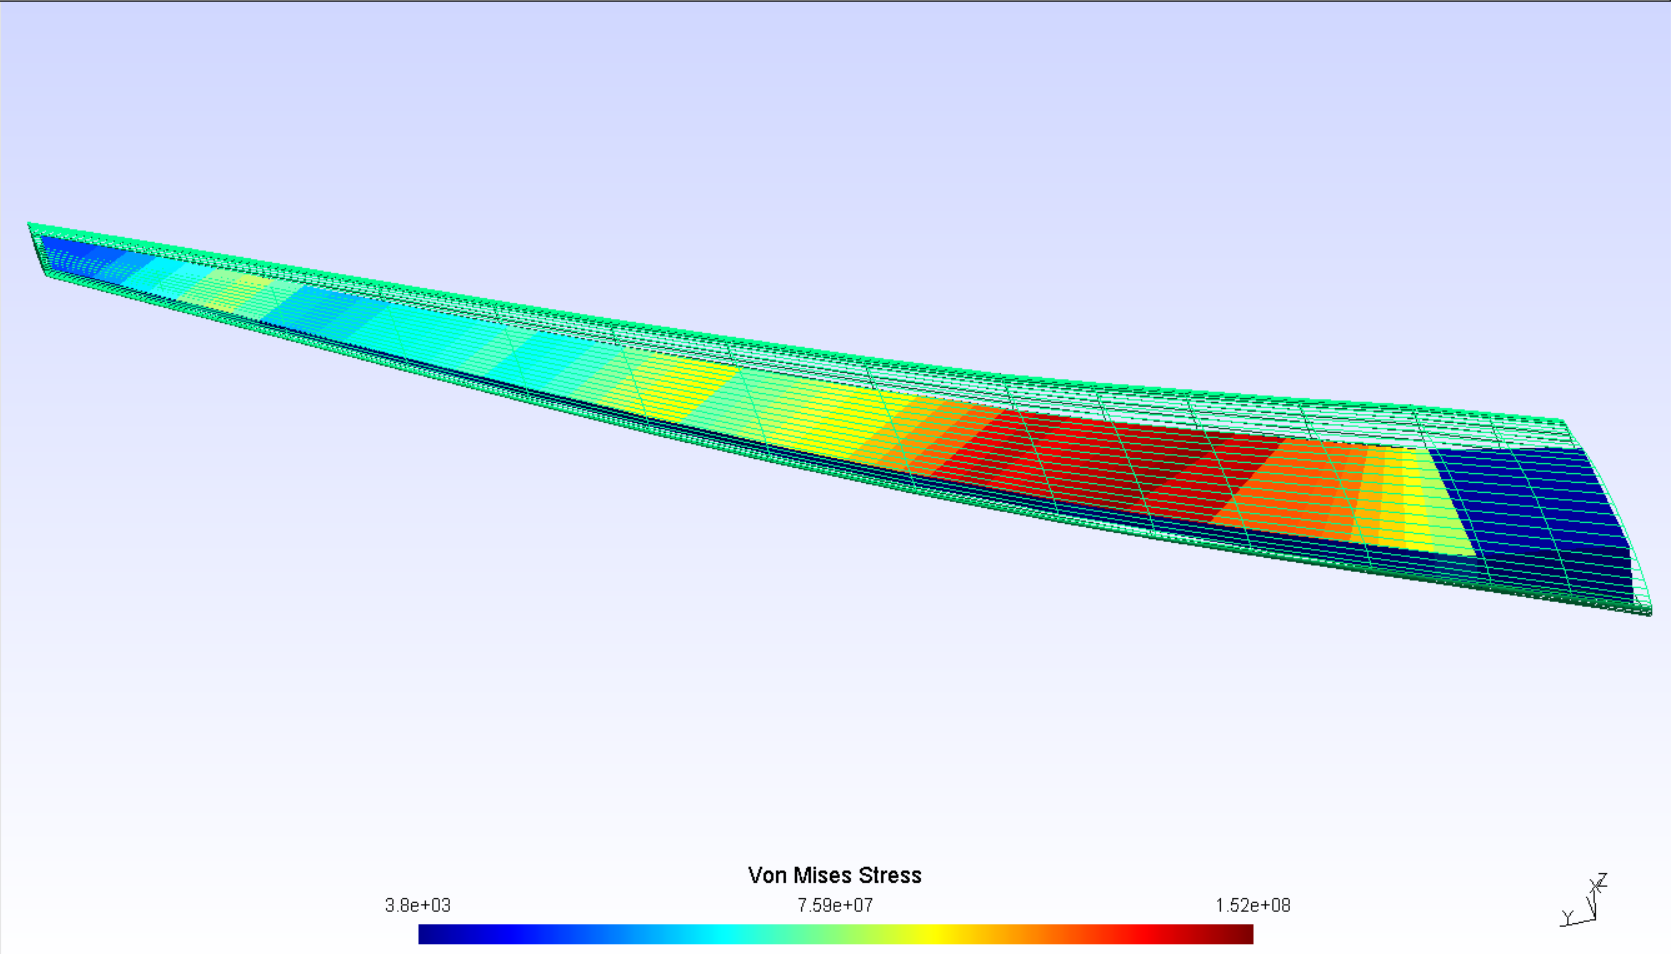
\includegraphics[width=\linewidth]{images/structure_aeromesh.PNG}
    \caption{Von Mises stress [Pa] on the structural mesh, aerodynamic mesh shown for reference.}
    \label{fig:structure_aeromesh}
\end{figure}

\section{Preliminary results}
\label{sec:results}

The sample problem was set up using the low-fidelity solver (PANAIR) and NASTRAN. Some slight changes were made on the original scripts to ensure compatibility with newer versions of Python. However, the overall strategy did not change. An optimal solution is found after 286 iterations for a $C_{d_i}=0.00718$. The wing shape showing Von Mises stress is presented in fig. \ref{fig:structure_aeromesh}, the Cp distribution was also obtained. An equivalent implementation of the problem using a High-Fidelity solver (ADFlow) was also reviewed as a way to get familiar with its functioning. The computing time in this case is significantly larger compared to the previous one. \par
Other than the shape, stresses and $C_p$, it is possible to obtain plots of the solution monitor parameters, such as constraint convergence and overall optimization convergence. This information is important because it allows to establish criteria to manage the interaction between both fidelities of the program. A convergence plot of the sample problem in low fidelity mode is shown in fig.  \ref{fig:conv_plot}.

\begin{figure}[H]
    \centering
    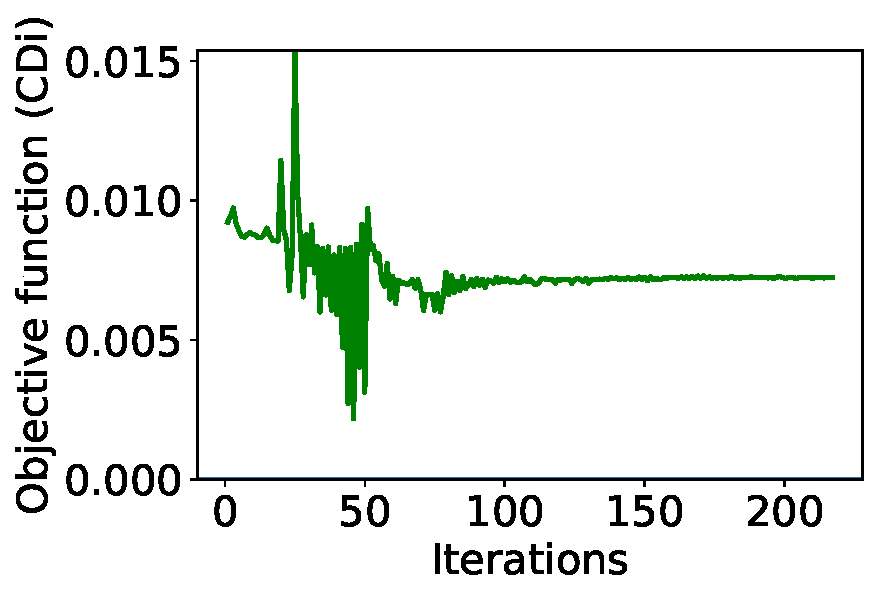
\includegraphics[width=0.8\linewidth]{images/objective_cdi.pdf}
    \caption{Convergence plot of the low fidelity optimization problem.}
    \label{fig:conv_plot}
\end{figure}

\section{Conclusions \& Future Work}
\label{sec:conclusions}
Up to this point, the main tasks of the present work were the state of the art review and the implementation of sample problems in Single-Fidelity mode in order to get acquainted with the various tools required to create the multifidelity optimization. Future work for S3 includes writing the python code that connects both fidelity levels within the OpenMDAO environment. This will allow the optimization of the sample case, which in turn can be used as a bench-marking reference to review the performance of the new proposal versus single-fidelity implementations. Depending on the results, minor or major changes will be applied to the multifidelity code in order to improve its efficiency. Once the method handles properly the sample case, a BWB configuration will be optimized and the results will be validated using academic sources. Since the complexity of the problem will increase, a second performance review of the code will be carried out to check for any possible improvements.   